\documentclass[../main.tex]{subfiles}
 
\begin{document}

% overview

This section describes the results achieved. Overall, the results indicate that the best models fit the non-expert's labels almost perfectly, but they also indicate -- as expected -- that the non-expert does not label maneuvers exactly like the expert.

% visual depiction of results

% this is in 3-Methodology.tex because I'm too lazy to learn how to place figures in LaTeX

% \begin{figure}
% \centerline{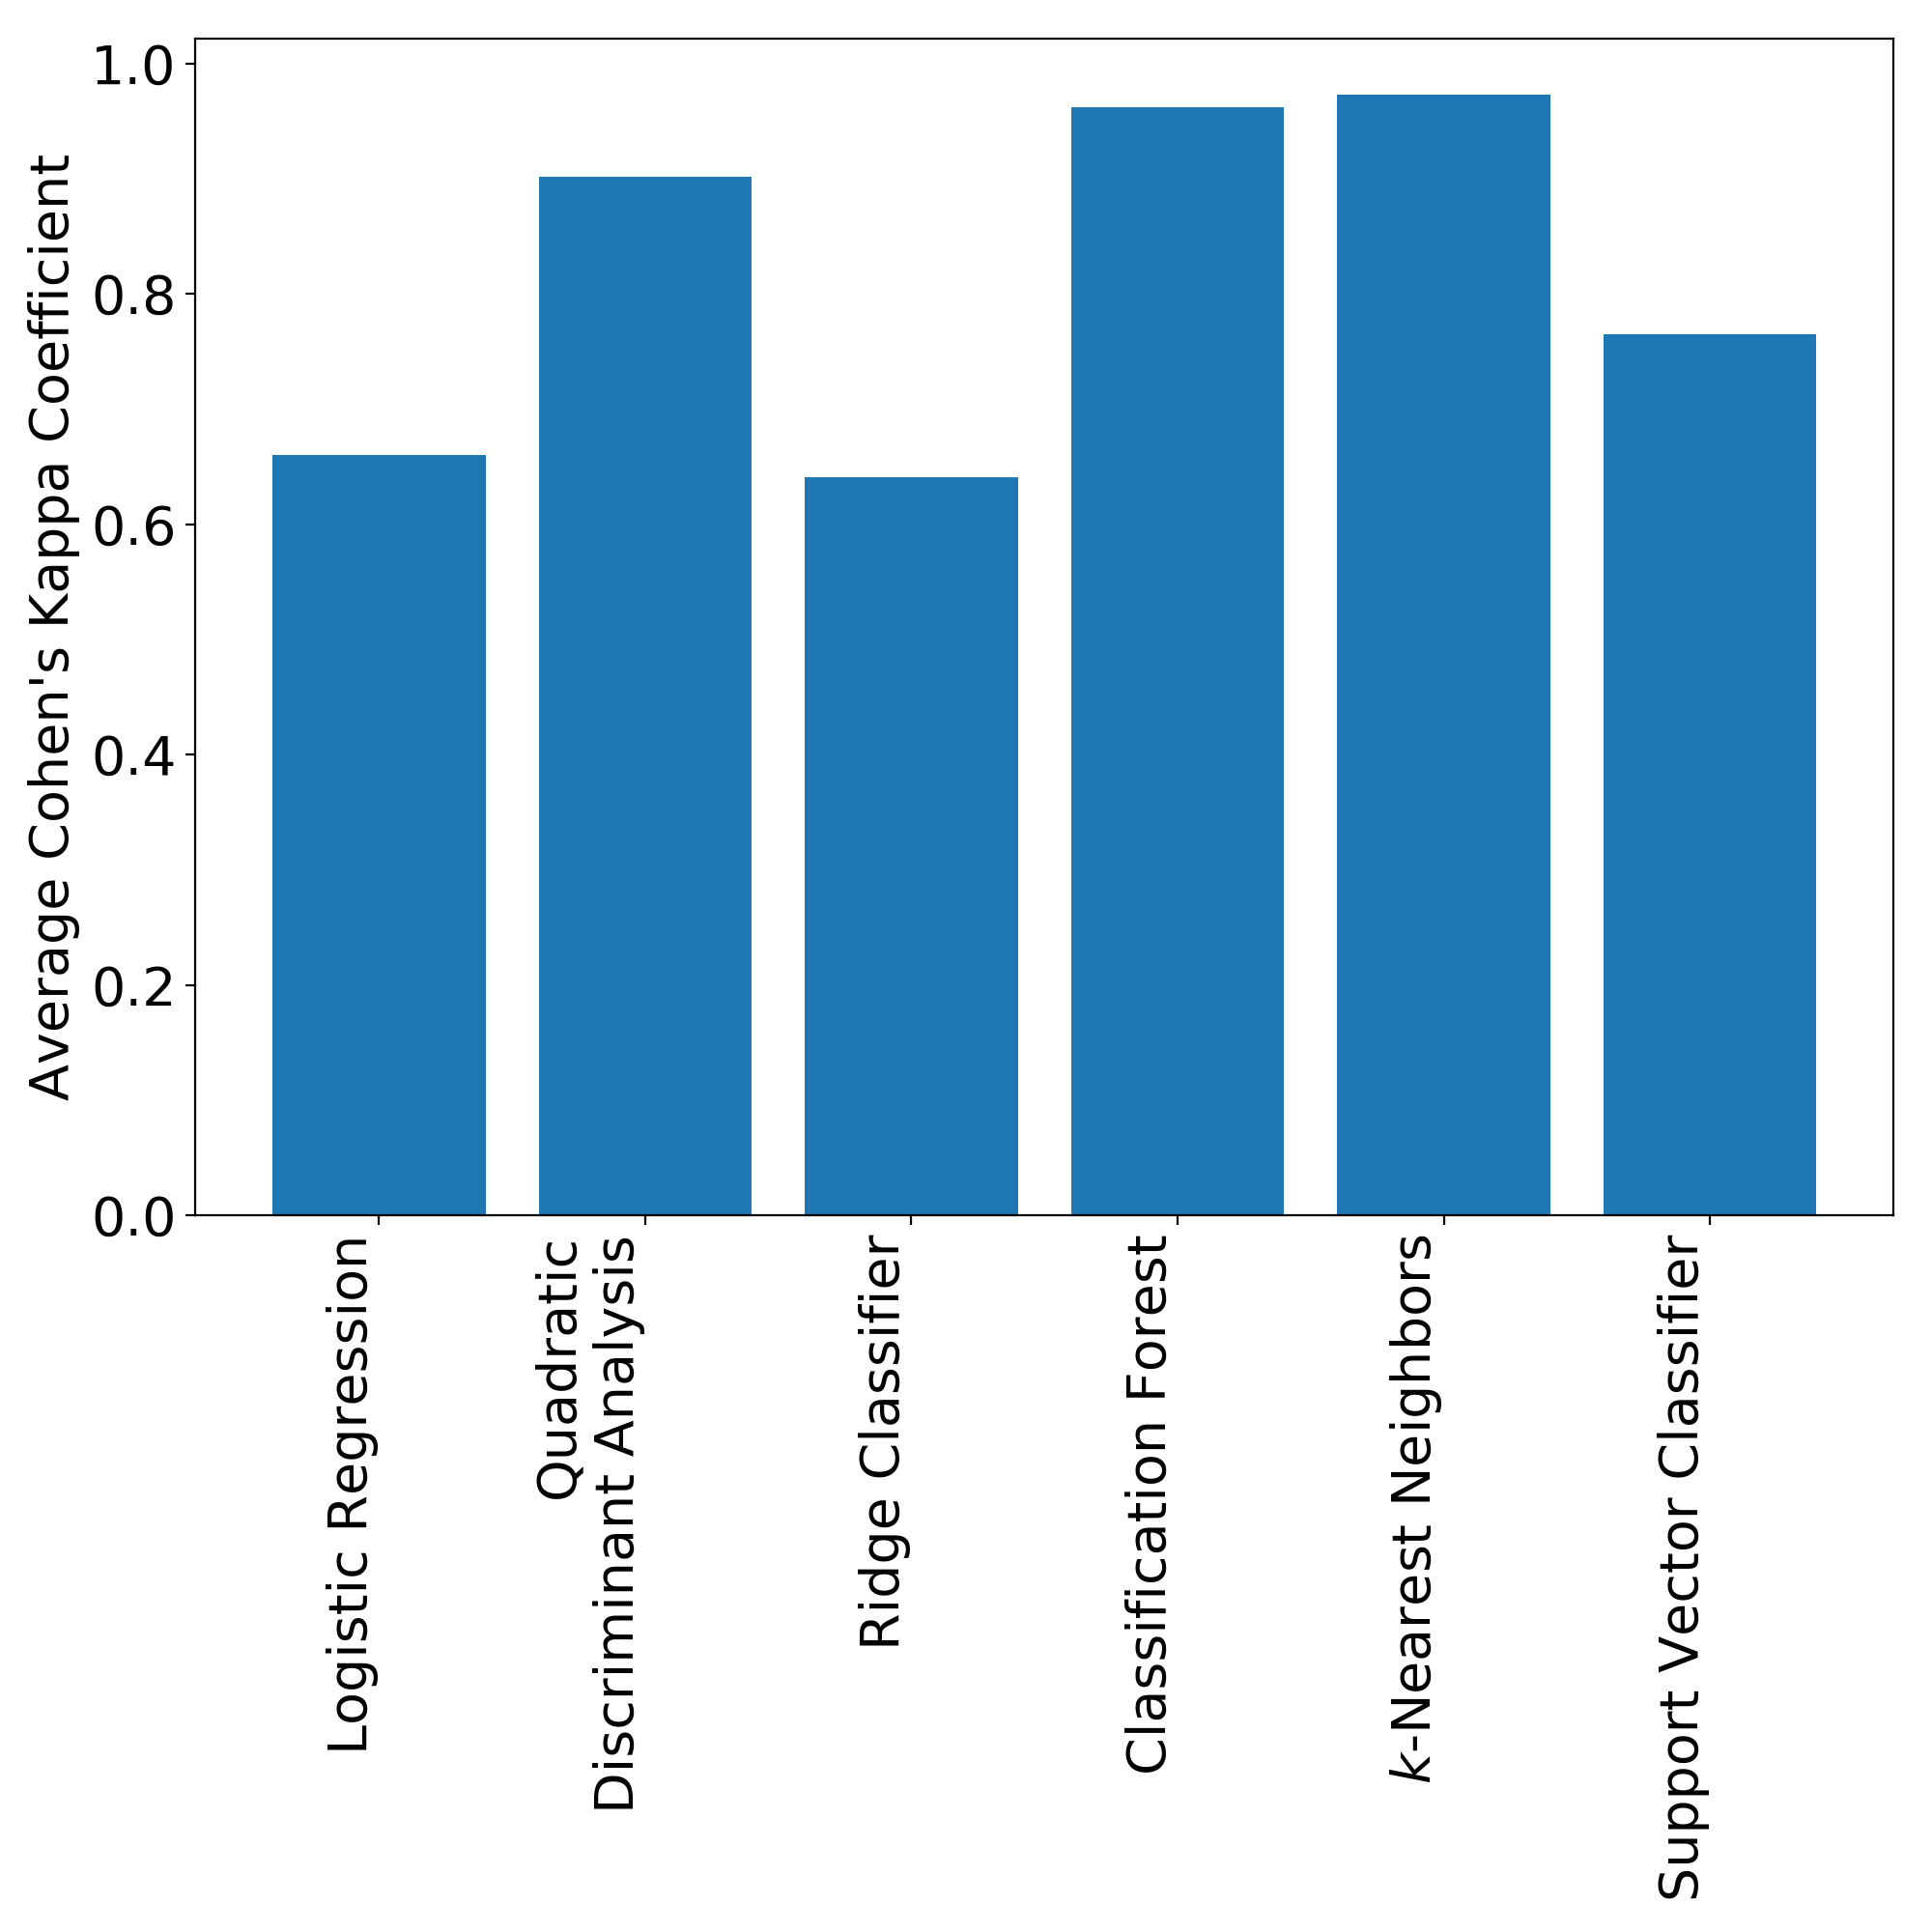
\includegraphics[width=\columnwidth]{ck-bar.png}}
% \caption{Cohen's kappa coefficient averaged over all parameter settings for each of the six types of classifier. These are the $\kappa$ values between models and the layman's labels, as computed on the training set during model fitting.}
% \label{fig:ck-bar}
% \end{figure}

\begin{table}
\caption{Cohen's Kappa Coefficient for Each Classifier}
\centering
\label{tab:score}
\begin{tabular}{|c|c|c|}
\hline
\textbf{Model}                  & \textbf{Layman} & \textbf{Expert} \\
\hline
Logistic Regression             & 0.696015        & 0.677175        \\
Quadratic Discriminant Analysis & 0.957674        & 0.927529        \\
Ridge Classification            & 0.657370        & 0.631847        \\
Classification Forest           & 0.996973        & 0.900345        \\
$k$-Nearest Neighbors           & 0.993946        & 0.897330        \\
Support Vector Classification   & 0.993946        & 0.897330        \\
\hline
\end{tabular}
\end{table}

\begin{table}
\caption{Accuracy for Each Classifier}
\centering
\label{tab:accuracy}
\begin{tabular}{|c|c|c|}
\hline
\textbf{Model}                  & \textbf{Layman} & \textbf{Expert} \\
\hline
Logistic Regression             & 0.802783        & 0.782977        \\
Quadratic Discriminant Analysis & 0.973443        & 0.951512        \\
Ridge Classification            & 0.777559        & 0.752535        \\
Classification Forest           & 0.997955        & 0.933480        \\
$k$-Nearest Neighbors           & 0.996134        & 0.931484        \\
Support Vector Classification   & 0.996134        & 0.931484        \\
\hline
\end{tabular}
\end{table}

\begin{table}
\caption{Cohen's Kappa Coefficient for Each Classifier When Roll, Pitch, and Yaw Features Are Excluded}
\centering
\label{tab:score-restricted}
\begin{tabular}{|c|c|c|}
\hline
\textbf{Model}                  & \textbf{Layman} & \textbf{Expert} \\
\hline
Logistic Regression             & 0.656764        & 0.637979        \\
Quadratic Discriminant Analysis & 0.739439        & 0.719577        \\
Ridge Classification            & 0.587684        & 0.564931        \\
Classification Forest           & 0.993946        & 0.897330        \\
$k$-Nearest Neighbors           & 0.984867        & 0.894308        \\
Support Vector Classification   & 0.993946        & 0.897330        \\
\hline
\end{tabular}
\end{table}

\begin{table}
\caption{Accuracy for Each Classifier When Roll, Pitch, and Yaw Features Are Excluded}
\centering
\label{tab:accuracy-restricted}
\begin{tabular}{|c|c|c|}
\hline
\textbf{Model}                  & \textbf{Layman} & \textbf{Expert} \\
\hline
Logistic Regression             & 0.775670        & 0.756660        \\
Quadratic Discriminant Analysis & 0.835090        & 0.813799        \\
Ridge Classification            & 0.729184        & 0.707838        \\
Classification Forest           & 0.996134        & 0.931484        \\
$k$-Nearest Neighbors           & 0.990283        & 0.929341        \\
Support Vector Classification   & 0.996134        & 0.931484        \\
\hline
\end{tabular}
\end{table}

% performance described in text that references the visuals

\figurename \ \ref{fig:ck-bar} depicts the average performance of each of the six model types in fitting the layman's labels. Clearly, \ac{qda}, the classification forest, and \ac{knn} perform consistently well. As can be seen in Tables \ref{tab:score}, \ref{tab:score-restricted}, \ref{tab:accuracy}, and \ref{tab:accuracy-restricted}, \ac{svc} can perform extremely well, but \figurename \ \ref{fig:ck-bar} shows that the poorest versions of \ac{svc} significantly decrease its average performance.

Table \ref{tab:score} contains the $\kappa$ values between the best version of each model (e.g., \ac{knn} when $k=1$ or the ridge when $\alpha=1.274275$) and the non-expert's labels. The table also contains the $\kappa$ value between the best version of each model and the expert's labels.

For completeness, and to compare Cohen's $\kappa$ coefficient to statistical accuracy, the accuracy scores between the best version of each model and the non-expert's labels and between the best version of each model and the expert's labels are shown in Table \ref{tab:accuracy}. As expected, the accuracy scores are higher than the respective $\kappa$ coefficients; this is because accuracy does not consider the possibility of chance agreement.

Tables \ref{tab:score-restricted} and \ref{tab:accuracy-restricted} are much like Tables \ref{tab:score} and \ref{tab:accuracy}, but all models in Tables \ref{tab:score-restricted} and \ref{tab:accuracy-restricted} are fit without roll, pitch, and yaw data. Some restricted models, like the classification forest, \ac{knn}, and \ac{svc}, perform much like they do when orientation data is included. The remaining models -- logistic regression, \ac{qda}, and the ridge -- perform noticeably worse. Each restricted model is certainly able to fit the layman's labels better than the expert's, but, again, the difference in $\kappa$ values is less than expected.

% performance discussed in text – did it work well? why or why not?

Depending on the type of model used, one can clearly fit a near-perfect model to the layman's labels, even if roll, pitch, and yaw data are excluded. When all features are included, the classification forest approach outperforms all others. We suspect this is due to the nature of the labels in question. One can easily rule out possible classes for a given observation using limited information. For example, a low roll value means that the aircraft is not turning; one can then easily evaluate altitude and airspeed to decide between \textit{takeoff} and \textit{cruise}.

A high-performing model, however, is not likely to predict the expert's labels quite as well. In fact, the best models are $10\%$ more likely to correctly predict the layman's labels than they are to correctly predict the expert's labels. This may indicate a degree of unreliability in the layman's labels.

Still, because some classification models fit the layman's labels so well, and because an expert is likely to be more consistent than a layman in labeling maneuvers, we assert that a classification model can also fit an expert's labels. Such a model can then label flight data in place of expert labelers.

% transition paragraph

The final section discusses conclusions one can draw from the research and the results. Additionally, it considers potential avenues for future, related research.

\end{document}